
\documentclass{standalone}
% font set
\usepackage{ctex}
\usepackage{fontspec}
\usepackage[T1]{fontenc}
\usepackage[sc]{mathpazo}
\usepackage{anyfontsize}
\setmainfont{Source Serif 4}
\setsansfont{Source Sans 3}
\setmonofont{Menlo}
\setCJKmainfont[BoldFont=黑体-简 中等,ItalicFont=楷体-简 常规体]{宋体-简 常规体}

% colors
\usepackage[dvipsnames]{xcolor}
\definecolor{pku-red}{RGB}{139,0,18}
\usepackage{colortbl}
\newcommand{\light}[1]{\textcolor{Orchid}{#1}}
\newcommand{\contrastlight}[1]{\textcolor{TealBlue}{#1}}

% plots
\usepackage{tikz}
\usepackage{tikz-cd}
\usetikzlibrary{arrows}
\usetikzlibrary{arrows.meta,positioning,calc,3d}
\usepackage{pgfplots}
\pgfplotsset{compat=newest}
\tikzset{
    punkt/.style={
        rectangle,
        rounded corners,
        draw=black, very thick,
        minimum height=2em,
        inner sep=6pt,
        text centered,
        fill=gray!30
    }
}

% math package
\let\Bbbk\relax
\usepackage{amsmath}
\usepackage{mathrsfs}
\usepackage{amssymb}
\usepackage{amsfonts}
\usepackage{stmaryrd}
\usepackage{latexsym}
\usepackage{extarrows}
\SetSymbolFont{stmry}{bold}{U}{stmry}{m}{n}


% math notations
\newcommand{\LHS}{\mathrm{LHS}}
\newcommand{\RHS}{\mathrm{RHS}}
\newcommand{\Z}{\mathbb{Z}}
\newcommand{\N}{\mathbb{N}}
\newcommand{\R}{\mathbb{R}}
\newcommand{\Q}{\mathbb{Q}}
\newcommand{\C}{\mathbb{C}}
\newcommand{\E}{\mathbb{E}}
\renewcommand{\O}{\mathcal{O}}
\newcommand{\id}{\mathrm{id}}
\DeclareMathOperator*{\Span}{Span}
\DeclareMathOperator*{\im}{Im}
\DeclareMathOperator*{\rank}{rank}
\DeclareMathOperator*{\card}{card}
\DeclareMathOperator*{\grad}{grad}
\DeclareMathOperator*{\argmax}{argmax}
\DeclareMathOperator*{\epi}{epi}
\DeclareMathOperator*{\maximize}{maximize}
\DeclareMathOperator*{\minimize}{minimize}
\renewcommand{\d}{\mathrm{d}}
\newcommand{\Pow}{\mathcal{P}}
\newcommand{\cov}{\mathsf{Cov}}
\newcommand{\var}{\mathsf{Var}}
\newcommand{\Nor}{\mathcal{N}}
\newcommand{\U}{\mathcal{U}}
\renewcommand{\t}{\mathsf{T}}
\newcommand{\T}{\top}
\newcommand{\F}{\bot}
\newcommand{\norm}[1]{\left\|#1\right\|}
\newcommand{\inner}[2]{\left\langle{#1},{#2}\right\rangle}
\newcommand{\e}{\mathrm{e}}
\newcommand{\const}{\mathrm{const}}
\newcommand{\scB}{\mathscr{B}}
\newcommand{\scF}{\mathscr{F}}
\newcommand{\G}{\mathscr{G}}
\newcommand{\Exp}{\mathsf{Exp}}
\newcommand{\DExp}{\mathsf{DExp}}
\newcommand{\Lap}{\mathsf{Lap}}
\newcommand{\calP}{\mathcal P}
\newcommand{\calS}{\mathcal S}
\newcommand{\calF}{\mathcal F}
\newcommand{\calM}{\mathcal M}
\newcommand{\KL}{\mathrm{KL}}
\newcommand{\ReLU}{\mathsf{ReLU}}
\newcommand{\val}{\mathsf{val}}

\begin{document}

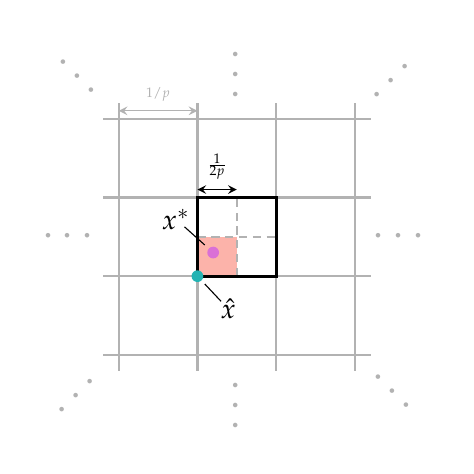
\begin{tikzpicture}[thick,>=stealth]

\draw[gray!60] (0,0) grid (3,3);
\draw[thick, gray!60] (3,0) -- (3.2,0);
\draw[thick, gray!60] (3,1) -- (3.2,1);
\draw[thick, gray!60] (3,2) -- (3.2,2);
\draw[thick, gray!60] (3,3) -- (3.2,3);

\draw[thick, gray!60] (0,3) -- (0,3.2);
\draw[thick, gray!60] (1,3) -- (1,3.2);
\draw[thick, gray!60] (2,3) -- (2,3.2);
\draw[thick, gray!60] (3,3) -- (3,3.2);

\draw[thick, gray!60] (0,0) -- (-0.2,0);
\draw[thick, gray!60] (0,1) -- (-0.2,1);
\draw[thick, gray!60] (0,2) -- (-0.2,2);
\draw[thick, gray!60] (0,3) -- (-0.2,3);

\draw[thick, gray!60] (0,0) -- (0,-0.2);
\draw[thick, gray!60] (1,0) -- (1,-0.2);
\draw[thick, gray!60] (2,0) -- (2,-0.2);
\draw[thick, gray!60] (3,0) -- (3,-0.2);

\node[scale=1.5, gray!60] at (3.6,1.5) {$\cdots$};
\node[scale=1.5, gray!60] at (-0.6,1.5) {$\cdots$};
\node[scale=1.5, rotate=90, gray!60] at (1.5,3.6) {$\cdots$};
\node[scale=1.5, rotate=90, gray!60] at (1.5,-0.6) {$\cdots$};
\node[scale=1.5, rotate=45, gray!60] at (3.5,3.5) {$\cdots$};
\node[scale=1.5, rotate=45, gray!60] at (-0.5,-0.5) {$\cdots$};
\node[scale=1.5, rotate=-45, gray!60] at (3.5,-0.5) {$\cdots$};
\node[scale=1.5, rotate=-45, gray!60] at (-0.5,3.5) {$\cdots$};

\filldraw[fill=Salmon,draw=none,opacity=0.6] (1,1) rectangle (1.5,1.5);

\draw[densely dashed, gray!60] (1.5,1) -- (1.5,2);
\draw[densely dashed, gray!60] (1,1.5) -- (2,1.5);

\draw[very thick] (1,1) -- (2,1) -- (2,2) -- (1,2) -- cycle;


\node[circle, fill=Orchid, inner sep=1.5pt] (x-star) at (1.2,1.3) {};
\node[above left=0.1cm and 0.1cm of x-star] (x-star-label) {$x^*$};
\draw[thin,shorten <= 0.4cm, shorten >=0.1cm] (x-star) -- (x-star-label);

\node[circle, fill=TealBlue, inner sep=1.5pt] (x-star) at (1,1) {};
\node[below right=0.1cm and 0.1cm of x-star] (x-star-label) {$\hat{x}$};
\draw[thin,shorten <= 0.35cm, shorten >=0.1cm] (x-star) -- (x-star-label);


\draw[<->,thin] (1,2.1) -- node[above,font=\tiny] {$\frac{1}{2p}$} (1.5,2.1);
\draw[<->,thin,gray!60] (0,3.1) -- node[above,font=\tiny] {$1/p$} (1,3.1);
\end{tikzpicture}

\end{document}
